\documentclass[letterpaper, 11pt]{article} 

\usepackage{graphics,graphicx}
\usepackage{multicol} 
\usepackage{parskip}
\usepackage{amsmath}
\usepackage{multirow}
\usepackage[utf8]{inputenc}
\usepackage{fancyhdr}
\usepackage[title]{appendix}
\usepackage{wasysym}
\usepackage{url}
\usepackage{subcaption}

\usepackage[font=footnotesize,labelfont=small]{caption}
\captionsetup{width=0.85\linewidth}

\RequirePackage{geometry}
\geometry{margin=2cm}

\setlength{\parskip}{0.2cm}
\setlength{\parindent}{0pt}


\title{Assignment 1: Multithreading and the Problem of False Sharing}
\author{
Tai Duc Nguyen \\
ECEC 622: Parallel Computer Architecture
}
\date{\today}

\begin{document}

\maketitle

\rule{\textwidth}{1pt}

\begin{abstract}
	In modern computing systems, CPUs often have multiple cores that can manage multiple threads. Mutithreading can accelerate the computing capabilities of many applications. One such application is called SAXPY, or Single-Precision A·X Plus Y: a scalar multiplies a vector, which is added to another vector. Variants of this extremely simple benchmark can test a system's computing and memory bandwidth. In this assignment, the problem of False Sharing is explored in multithreaded applications using SAXPY as the benchmark. 
\end{abstract}

\rule{\textwidth}{1pt}

\section{Experimental Setup}

In order to measure the effect of False Sharing, a baseline execution time is established by running SAXPY in a serial fashion (no False Sharing): looping through all N elements and do N operations $\bar{Y} = a \cdot \bar{X} + \bar{Y}$. 

Then, a multithreaded application is built such that N operations are chunked into T threads: thread i will operate on all elements from i*chunk\_size to i*chunk\_size*2. This \textbf{chunking method} can reduce the effect of False Sharing but may not do so completely because there is a chance that the cache line of each processor/thread is independent from one another; or, only overlap slightly.

Finally, another multithreaded application is created using the \textbf{striding method}: thread i will execute the operation above for element i, i + num\_threads, i + num\_threads*2, i + num\_threads*3... and so on. This will guarantee the effect of False Sharing because cache coherency is maintained on a cache-line basis, and not for individual elements. Hence, simultaneous updates of individual elements in the same cache line coming from different processors/threads invalidates entire cache lines every time the vector $\bar{Y}$ is updated by any processors/threads.

\textit{Note: running \texttt{make all} will generate the report in \texttt{rpt.txt}}

\section{Experimental Result}

\begin{figure}[htb!]
	\centering
	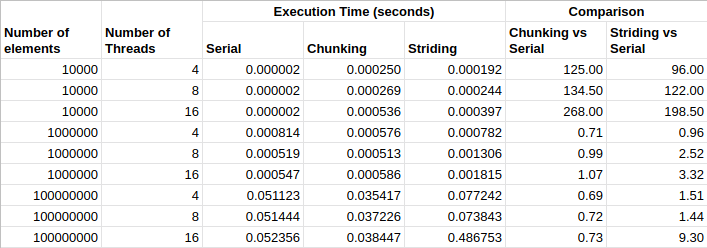
\includegraphics[width=1.0\linewidth]{result.png}
	\caption{Results of execution times for all 3 scenarios: Serial, Chunking, and Striding}
	\label{fig1}
\end{figure}

\newpage

\section{Discussion}

From Figure \ref{fig1}, it is apparent that multithreading only provides computational benefits at $N > 10^6$ elements. Below $10^6$, the overhead of threads, and their associated data structures made the total execution time much higher than doing things serially. At $N = 10^6$ elements, chunking provides some small benefits but not much due to some False Sharing is still present. Striding, however, does not provide any benefits due to false sharing. At $N = 10^8$ elements, same behaviors applies to both chunking and striding, excluding the case where $T = 16$ on striding. In this case, each thread has very little work, hence, False Sharing is magnified: every operation on any thread will cause the cache line to be invalidated.

\end{document}